
\documentclass{beamer}

%\usepackage{pstricks}

\usepackage{setspace}

\usepackage{amssymb}
\usepackage{textcomp}
\usepackage{tikz}
%%?\usepackage[backslant]{aurical}

%%?\usepackage{hanging}

%\usepackage{DejaVuSerif}

\usepackage{setspace}

\usepackage{microtype}
\usepackage{hyphenat}
%%?\usepackage{dashrule}
%\usepackage[usenames,dvipsnames]{xcolor}

\usetikzlibrary{arrows, positioning, shapes}
\usetikzlibrary{backgrounds}


%%?\usepackage{wrapfig}

\usetikzlibrary{arrows, positioning, shapes}

\usetheme{Singapore}
\setbeamertemplate{blocks}[rounded][shadow=true]
\setbeamertemplate{frametitle}[default][center]
\setbeamertemplate{caption}[numbered]

\setlength{\paperwidth}{10.in}
\setlength{\paperheight}{7.5in}
\setlength{\textwidth}{9.in}
\setlength{\textheight}{6.5in}

\newcommand{\cfbox}[2]{%
	\colorlet{currentcolor}{.}%
	{\color[rgb]{#1}%
		\fbox{\color{currentcolor}#2}}%
}


%%?\usecolortheme{spruce}

%\setbeamercolor{block title}{red}   
%\setbeamercolor{block title}{red}   

%%\usecolortheme{orchid}
%\usepackage{float}

%\setbeamerfont{itemize/enumerate body}{size=\small}
%\setbeamerfont{normaltext}{size=\}
%\setbeamerfont{block body}{size=\small}
\setbeamerfont{block title}{size=\large}
%\setbeamerfont{block body example}{size=\tiny}

\newcommand{\colortriangle}{{\color[rgb]{0.45, 0.4, 0.28}$\blacktriangleright$}}
	
\newcommand\FourQuad[4]{%
	
	\begin{minipage}[b][.45\textheight][t]{.47\textwidth}#1\end{minipage}\hfill%
	\begin{minipage}[b][.45\textheight][t]{.47\textwidth}#2\end{minipage}\\[0.5em]
	\begin{minipage}[b][.45\textheight][t]{.47\textwidth}#3\end{minipage}\hfill
	\begin{minipage}[b][.45\textheight][t]{.47\textwidth}#4\end{minipage}%
}

\newcommand\ThreeQuad[3]{%
	\hspace{2pt}\begin{minipage}[b][.23\textheight][c]{.99\textwidth}#1\end{minipage}\hfill%
	\begin{minipage}[b][.75\textheight][t]{.55\textwidth}#2\end{minipage}\hfill
	\begin{minipage}[b][.75\textheight][t]{.43\textwidth}#3\end{minipage}%
}

\newcommand\TwoQuad[2]{%
	\begin{minipage}[b][.75\textheight][t]{.55\textwidth}#1\end{minipage}\hfill
	\begin{minipage}[b][.75\textheight][t]{.43\textwidth}#2\end{minipage}%
}

\newcommand\OneQuad[1]{%
	\begin{minipage}[b][.45\textheight][t]{1.01\textwidth}#1\end{minipage}\hfill
	%\begin{minipage}[b][.75\textheight][t]{.43\textwidth}#2\end{minipage}%
}


\newenvironment{quadblock}[1]{\begin{block}{\begin{center}\Large{%
\colorbox[rgb]{0.25,0.1,0.25}{\color{yellow}{\textbf{#1}}}
}\end{center}}%
\begin{minipage}[c]{.97\textwidth}\vspace{1em}
}{
\end{minipage}
\end{block}}


\newenvironment{mpblock}[1]{\begin{block}{\begin{center}\Large{%
\colorbox[rgb]{0.25,0.1,0.25}{\color{yellow}{\textbf{#1}}}
}\end{center}}%
\begin{minipage}[c]{.97\textwidth}\vspace{1em}
\begin{textsf}}{\end{textsf}
\end{minipage}
\end{block}}

%%?\usepackage{pbsi}
%\usepackage{oesch}
%\usepackage{LobsterTwo}

%\newcommand{\doubleCenteredFramebox}[1]{%
%\begin{center}%
%\framebox{%
%\begin{minipage}{0.85\textwidth}\begin{center}%
%#1\end{minipage}\end{center}}\end{center}}

%\setlength{\fboxsep}{0.15em}



\newcommand{\doubleCenteredFramebox}[1]{%
\setlength{\fboxsep}{2em}\setlength{\fboxrule}{2pt}
\begin{center}\cfbox{0.1, 0.5, 0.8}{\begin{minipage}{0.85\textwidth}\begin{center}\setlength{\fboxsep}{.25em}#1
	\end{center}\end{minipage}}\end{center}}


\newcommand{\halfPageFramebox}[1]{%
	\setlength{\fboxsep}{2em}\setlength{\fboxrule}{1pt}
	\begin{center}\cfbox{0.1, 0.5, 0.8}{\begin{minipage}{0.5\textwidth}\begin{center}\setlength{\fboxsep}{.25em}#1
				\end{center}\end{minipage}}\end{center}}

\newcommand{\sfitem}[1]{\item \LARGE{\textbf{\textsf{#1}}}}				

\renewcommand*\rmdefault{cmfib}

\newcommand{\scitem}[1]{\item {\Large{{\fontfamily{pag}\selectfont \textbf{#1}}}}}			
\newcommand{\smscitem}[1]{\item {\small{{\fontfamily{pag}\selectfont \textbf{#1}}}}}			


\newcommand{\embitem}[1]{\item \textbf{{\large #1}}}			


\newcommand{\highlightframebox}[1]{\cfbox{1,.5,1}{#1}}

%\begin{minipage}[.45\textheight][t]}{\end{minipage}\end{block}}

\newcommand{\manyasciimacron}{\textasciimacron\textasciimacron\textasciimacron%
\textasciimacron\textasciimacron\textasciimacron\textasciimacron\textasciimacron\textasciimacron%
\textasciimacron\textasciimacron\textasciimacron\textasciimacron\textasciimacron\textasciimacron%
\textasciimacron\textasciimacron\textasciimacron\textasciimacron\textasciimacron\textasciimacron%
}

\newcommand{\manyemdash}{\texttwelveudash\texttwelveudash\texttwelveudash\texttwelveudash\texttwelveudash%
 \texttwelveudash\texttwelveudash\texttwelveudash\texttwelveudash\texttwelveudash\texttwelveudash\texttwelveudash%
 \texttwelveudash\texttwelveudash\texttwelveudash\texttwelveudash\texttwelveudash\texttwelveudash\texttwelveudash%
}


\newenvironment{lightquadblock}[1]{\begin{center}\LARGE{%
			\colorbox[rgb]{.99,.99,0.66}{\color[rgb]{.14,.14,.04}{\hspace{-1em}\makebox[\textwidth]{#1}}}
		}\end{center}
		%\begin{framebox}
		\begin{minipage}[c]{.9\textwidth}\vspace{1em}
		}{
	\end{minipage}}
	
	
	\newenvironment{lightqblock}[1]{\begin{center}\LARGE{%
				\colorbox[rgb]{.90,.90,0.90}{\cfbox{.96,.94,.96}{\color[rgb]{.2,.06,.04}{\hspace{-1em}\makebox[\textwidth]{#1}}}}
			}\end{center}
			%\begin{framebox}
			\begin{minipage}[c]{.99\textwidth}\vspace{1em}
			}{
		\end{minipage}}
		

\newcommand\TwoQuadV[4]{%
	\begin{minipage}[b][.20\textheight][t]{1.04\textwidth}\begin{lightqblock}{#1}#2\end{lightqblock}\end{minipage}
	\begin{center}\begin{minipage}[t][.78\textheight][t]{.9\textwidth}%
		\begin{quadblock}{#3}\begin{minipage}{\textwidth}#4\end{minipage}\end{quadblock}\end{minipage}\end{center}%
}


%\newcommand{\conversationPatterns}{\framebox{%
%Conver\-\\
%sation\\
%Patterns}}

\newcommand{\conversationPatterns}{	
\begin{minipage}{32pt}\centering{\begin{scriptsize}\textbf{Convers\-ation\\Patterns}\end{scriptsize}} 
\end{minipage}}

\newcommand{\q}[1]{``#1"}


\definecolor{lqboutercolor}{rgb}{.93,.91,.92}
\definecolor{lqbinnercolor}{rgb}{.98,.98,.98}

\definecolor{blGreen}{rgb}{.2,.7,.3}
\definecolor{darkRed}{rgb}{.2,.0,.1}

\definecolor{postLinkColor}{rgb}{.5,.5,.1}

\definecolor{fcBoxColor}{rgb}{.8,.6,.3}

\definecolor{BlueGreen}{rgb}{.1,.6,.4}

\newenvironment{postfragment}{\begin{minipage}{5.4cm}\begin{small}}
{\end{small}\end{minipage}}

\newenvironment{postComment}{\begin{minipage}{8cm}\begin{small}}
{\end{small}\end{minipage}}

\newenvironment{postLongComment}{\begin{minipage}{9cm}\begin{small}}
		{\end{small}\end{minipage}}


\newenvironment{tightcenter}{%
	\setlength\topsep{0pt}
	\setlength\parskip{0pt}
	\begin{center}
	}{%
\end{center}
}

\newcommand{\tightcenterline}[1]{\begin{tightcenter}#1\end{tightcenter}}



\definecolor{postBkgColor}{rgb}{.95,.85,.95}
\definecolor{postCommentBkgColor}{rgb}{.85,.85,.95}

\definecolor{grammarArrowColor}{rgb}{.85,.85,.45}

\tikzstyle{postStyle}=[draw=yellow!120,rounded corners,fill=postBkgColor,thin,inner sep=.2cm]
\tikzstyle{postCommentStyle}=[draw=postCommentBkgColor,double,fill=postCommentBkgColor,thick,inner sep=.2cm]

\tikzstyle{sdComponent}=[double,rounded corners,draw=brown!120,fill=blue!50,thin,inner sep=.2cm]
\tikzstyle{cnvComponent}=[double,shape=diamond,rounded corners,draw=brown!120,fill=blue!50,thin,inner sep=0cm]

\tikzstyle{baseStyle}=[fill=purple!50,draw=cyan!20,ultra thick,double,shape=diamond,inner sep=.15cm]
\tikzstyle{componentStyle}=[fill=red!50,draw,shape=ellipse,inner sep=.15cm]

\tikzstyle{componentExtendedStyle}=[fill={rgb:red,10;green,10;blue,2},draw,shape=rectangle,inner sep=.15cm]

\newcommand{\emphcolor}{%
	\colorlet{currentcolor}{.}%
	\color[rgb]{.4,.4,.4}}

\newcommand{\ncolor}{%
	\color{currentcolor}}


\definecolor{slidePartHeadColor}{rgb}{0,.2,.1}

\newcommand{\slidePartHead}[1]{{\fontfamily{pnc}\selectfont\color{slidePartHeadColor}\LARGE#1}}

\newcommand{\slidePartHeadCenter}[1]{\slidePartHead{\begin{minipage}{\textwidth}\begin{center}#1\end{center}\end{minipage}}}

\newcommand{\componentLabel}[1]{\begin{minipage}{3.5cm}\begin{center}#1\end{center}\end{minipage}}
\newcommand{\baseComponentLabel}[1]{\begin{minipage}{2cm}\textbf{\begin{center}#1\end{center}}\end{minipage}}

\newcommand{\componentExtendedLabel}[1]{\begin{minipage}{10cm}\begin{center}\textbf{#1}\end{center}\end{minipage}}

\newcommand{\cstd}[1]{\textbf{{\color[rgb]{.4,.4,.1}#1}}}

\usepackage{setspace}

%\fontfamily{pag}\selectfont \textbf{
\newcommand{\raiseBoxL}[1]{\makebox{\raisebox{.1em}{{\fontfamily{put}\fontseries{sb}\selectfont #1}\hspace{1.2em}}}}
%	\begin{textsf}{\small}{}\end{textsf}\end{minipage}}

\newcommand{\doubleFrame}[1]{%
\fcolorbox{fcBoxColor!50}{gray!50}{
%{\begin{center}
\begin{minipage}{.98\textwidth}
%\begin{center}	
\hspace{9pt}\vspace*{2pt}		
\fcolorbox{fcBoxColor!90}{white}{%
\begin{minipage}{.96\textwidth}%
\begin{center}\begin{minipage}{.94\textwidth}				
\begin{spacing}{1}\vspace{1em}\part{title}#1\end{spacing}%
\end{minipage}\end{center}
\end{minipage}}
%\end{center}
\end{minipage}}
%\end{center}}
}%


\newcommand{\doubleFrameTwo}[2]{%
\begin{center}
\begin{minipage}{\textwidth}	
\fcolorbox{fcBoxColor!50}{gray!50}{
%	\begin{center}
\begin{minipage}{\textwidth}
	\begin{center}
			%\hspace{4pt}\vspace*{2pt}		
			\fcolorbox{fcBoxColor!90}{white}{%
				\begin{minipage}{.95\textwidth}%
\begin{center}\begin{minipage}{.91\textwidth}#1\end{minipage}\end{center}%
				\end{minipage}}\vspace*{.5em}\\
%\vspace*{2pt}
%\hspace{4pt}				
\fcolorbox{fcBoxColor!90}{white}{
		\begin{minipage}{.94\textwidth}
\begin{center}\begin{minipage}{.91\textwidth}#2\end{minipage}\end{center}%
		\end{minipage}}
\end{center}		
\end{minipage}
%
}\par 
\end{minipage}
\end{center}		
}

\newcommand{\itup}[1]{\raisebox{2pt}{{\normalsize(#1)}}}

\newcommand{\FER}{{\color[rgb]{0.1,0.25,0.6}{FER}}}
\newcommand{\BER}{{\color[rgb]{0.1,0.25,0.6}{BER}}}
\newcommand{\IR}{{\color[rgb]{0.1,0.25,0.6}{IR}}}

\newcommand{\FrontEnd}{{\color[rgb]{0.1,0.25,0.6}{Front-End}}}
\newcommand{\BackEnd}{{\color[rgb]{0.1,0.25,0.6}{Back-End}}}
\newcommand{\Intermediate}{{\color[rgb]{0.1,0.25,0.6}{Intermediate}}}

%\newcommand{\doubleFrameTwo}[2]{%
%\fcolorbox{fcBoxColor}{gray!50}{
%\begin{minipage}{.98\textwidth}
%\hspace{4pt}\vspace*{2pt}	
%\fcolorbox{fcBoxColor}{white}{%
%\begin{minipage}{.95\textwidth}#1
%\end{minipage}}#1
%\fcolorbox{fcBoxColor}{white}{%
%\begin{minipage}{.95\textwidth}#2%
%\end{minipage}}
%}


%\newenvironment{doubleFrame}{%
%\fcolorbox{fcBoxColor}{gray!50}{\begin{minipage}{\textwidth}}
%{\end{minipage}}}

%\newenvironment{doubleFrame}{% \fcolorbox{fcBoxColor}{gray!50}{%
%\fbox{\begin{minipage}{\textwidth}%
%}
%{\end{minipage}}}
%}}

%\newcommand{\doubleFrame}[1]
\newcommand{\nodeincludegraphics}[2][0.8\textwidth]{
\node[anchor=south west,inner sep=0] (image) at (0,0){%
\includegraphics[width=#1]{#2}};}

\newcommand{\nodeincludegraphicsR}[2][1]{
\node[anchor=south west,inner sep=0] (image) at (0,0){%
\includegraphics[scale=#1]{#2}};}

\newcommand{\nodeincludegraphicsAS}[1]{
\node[anchor=south west,inner sep=0] (image) at (0,0){%
\includegraphics{#1}};}

\newcommand{\nodeincludegraphicsTR}[3]{
\node[anchor=south west,inner sep=0] (image) at (0,0){%
\includegraphics[trim={0 #2 #1 0},clip]{#3}};}

\newcommand{\ann}[9]{%
\path [draw=#1,draw opacity=#2,line width=#3, fill=#4, fill opacity = #5, even odd rule] %
(#6) ellipse(#7 and #8) ellipse(#7*#9 and #8*#9);}

\makeatletter
\newcommand*\getX[1]{\expandafter\getX@i#1\@nil}
\newcommand*\getY[1]{\expandafter\getY@i#1\@nil}
\def\getX@i#1,#2\@nil{#1}
\def\getY@i#1,#2\@nil{#2}
\makeatother

\newcommand{\rectann}[9]{%
\path [draw=#1,draw opacity=#2,line width=#3, fill=#4, fill opacity = #5, even odd rule] %
(#6) rectangle(\getX{#6}+#7,\getY{#6}+#8)
({\getX{#6}+((#7-(#7*#9))/2)},{\getY{#6}+((#8-(#8*#9))/2)}) rectangle %
({\getX{#6}+((#7-(#7*#9))/2)+#7*#9},{\getY{#6}+((#8-(#8*#9))/2)+#8*#9});}

\newcommand{\rectanneatdbl}[9]{%
\path [draw=#1,draw opacity=#2,line width=#3, fill=#4, fill opacity = #5, even odd rule] %
(#6) rectangle(\getX{#6}+#7,\getY{#6}+#8)
({\getX{#6}+\getX{#9}},{\getY{#6}+\getY{#9}}) rectangle %
({\getX{#6}+#7-\getX{#9}},{\getY{#6}+#8-\getY{#9}})
;}

\newcommand{\rectanneat}[9]{%
\path [draw=#1,draw opacity=#2,line width=#3, fill=#4, fill opacity = #5, even odd rule] %
(#6) rectangle(\getX{#6}+#7,\getY{#6}+#8)
({\getX{#6}+(#7/abs(#7))*#9},{\getY{#6}+(#8/abs(#8))*#9})
rectangle({\getX{#6}+#7-(#7/abs(#7))*#9},{\getY{#6}+#8-(#8/abs(#8))*#9});}

\newcommand{\colorarr}[8]{
\draw [#1, draw=#2,draw opacity=#3,
fill=#4,fill opacity=#5,line width=#6] (#7) to (#8);
}

%({\getX{#6}+(\getX{#6}/abs(\getX{#6}))*#9},{\getY{#6}+(\getY{#6}/abs(\getY{#6}))*#9}) %
%rectangle ({\getX{#6}+#7+(\getX{#6}/abs(\getX{#6}))*#9},%
%{\getY{#6}+#8+(\getY{#6}/abs(\getY{#6}))*#9})
%;}

%%({\getX{#6}+#7-(\getX{#6}/abs(\getX{#6}))*#9},{\getY{#6}+#8-(\getY{#6}/abs(\getY{#6}))*#9})

%%\path [draw=#1,draw opacity=#2,line width=#3, fill=#4, fill opacity = #5] %
%%({\getX{#6}+((#7-(#7*#9))/2)},{\getY{#6}+((#8-(#8*#9))/2)}) rectangle %
%%({\getX{#6}+((#7-(#7*#9))/2)+#7*#9},{\getY{#6}+((#8-(#8*#9))/2)+#8*#9});}

%%((#7-(#7*#9))/2)
%%(\getX{#6}+(#7-(#7*#9))/2,\getY{#6}+(#8-(#8*#9)/2))


%(\getX{#6}+(#7-(#7*#9))/2,\getY{#6}+(#8-(#8*#9)/2)) 
%rectangle(\getX{#6}+#7*#9,\getY{#6}+#8*#9)
%;}

%\documentclass{pstricks}
\begin{document}
%
\begin{frame}{\ft{Loading the document ...}}

SLIDE 1

\end{frame}




%
\begin{frame}{\ft{Loading the document ...}}

SLIDE 2

\end{frame}



%

\begin{frame}{\ft{Using Custom Viewers}}

\doubleFrame{Re-PDF data is delivered to potential 
buyers embedded in PDF files so that buyers can open 
these files even if they do not have the Re-PDF software.  
As a result, users will not be burdened with files that 
they cannot open or identify.  At the same time, 
users that \textit{do} install the Re-PDF viewer will 
experience the Re-PDF presentations interactively --- adding 
many layers to the ordinary PDF experience.}

\begin{tikzpicture}
%\nodeincludegraphics[0.88\textwidth]{screenshots/ss-norpdf.png}
\nodeincludegraphicsTR{2.5cm}{2cm}{screenshots/ss-norpdf.png}

\ann{darkRed}{0.7}{1mm}{grammarArrowColor}{0.5}{6,3.5}{6.5}{1}{0.85}
%\node [anchor=west] (note) at (-1,3) {\Large Note};
%\draw [-latex, ultra thick, red] (note) to[out=0, in=-120] (0.48,0.80);

 \node [anchor=west,fill=blue!20!yellow,inner sep=13, text width=14cm]
  (longnote) at (1.5,1.5) {%  %{\color{rb!85!red}{
  {\cframedboxyellow{\large \textbf{Re-PDF documents include links 
  to web pages where users can download each 
  realtor's customized version of the Re-PDF viewer 
  --- for users who are reading the 
  document with other PDF applications.}}}};


\end{tikzpicture}


\end{frame}


%

\begin{frame}{\ft{Launching Dialog Windows}}

\doubleFrame{By clicking on links in Re-PDF documents, 
users can launch dialog windows with 
special layout and features.  For 
regular PDF viewers, these links will take users to 
realtors\curlyapos{} web pages.  However, for custom Re-PDF viewers, 
these links will open adjunct viewers --- fine-tuned for 
each realtor --- such as customized dialog boxes 
and 3D or multimedia presentations.}

\begin{tikzpicture}
%\nodeincludegraphics[0.87\textwidth]{screenshots/ss-links.png}
\nodeincludegraphicsTR{2.5cm}{2cm}{screenshots/ss-links.png}

\node [anchor=west,fill=orange!8!white,inner sep=12, 
opacity=0.88, text opacity=1] (note) at (9.5,8.5) {\hc{Links}};

%\rectann{darkRed}{0.7}{1mm}{grammarArrowColor}{0.5}{2,8}{5}{-7}{0.5}
\rectanneat{darkRed}{0.7}{1mm}{grammarArrowColor}{0.5}{0,10}{9}{-7}{0.7}

%\draw [-latex, ultra thick, red] (note) to (7, 7);

\colorarr{>=latex, ->}{fcBoxColor!60!black}{0.8}{blGreen!30!red}{1}{1mm}{note}{7, 8}


 \node [anchor=west,fill=brown!20!white,inner sep=7, text width=10cm]
  (longnote) at (8.5,7) {%  %{\color{rb!85!red}{
  {\cframedbox{\large \textbf{Photo View Dialog (slides 9-12)}}}};

\colorarr{>=latex, ->}{fcBoxColor!20!black}
{0.8}{darkRed!70!blue}{2}{1mm}{longnote.west}{6.3, 7.5}


 \node [anchor=west,fill=brown!20!white,inner sep=7, text width=10cm]
  (longnote) at (8.5,5) {%  %{\color{rb!85!red}{
  {\cframedbox{\large \textbf{Virtual Tour Dialog (slides 16-17)}}}};

\colorarr{>=latex, ->}{fcBoxColor!20!black}
{0.8}{darkRed!70!blue}{2}{1mm}{longnote.west}{6.1, 6.8}



 \node [anchor=west,fill=brown!20!white,inner sep=7, text width=10cm]
  (longnote) at (8.5,3) {%  %{\color{rb!85!red}{
  {\cframedbox{\large \textbf{Room Dialog (slides 13-15)}}}};

\colorarr{>=latex, ->}{fcBoxColor!20!black}
{0.8}{darkRed!70!blue}{2}{1mm}{longnote.west}{5.9, 4.7}


%\draw [-latex, draw=darkRed,draw opacity=0.8,line width=#4] #5 to #6;


%[out=120, in=0]
\end{tikzpicture}


\end{frame}


%

\begin{frame}{\ft{Using Context Menus}}

\doubleFrame
}

\begin{tikzpicture}
%\nodeincludegraphics[0.87\textwidth]{screenshots/ss-contextmenu.png}

\nodeincludegraphicsTR{5.5cm}{2cm}{screenshots/ss-contextmenu.png}

\rectann{red}{0.3}{3mm}{blue!50!cyan}{0.5}{8.5,9}{7.5}{-6.5}{0.85}

\end{tikzpicture}


\end{frame}



%

\begin{frame}{\ft{The Photo Viewer}}

\doubleFrame{Re-PDF provides a suite of useful dialog boxes 
and a toolkit for programming customized presentations according 
to the preferences of each realtor.  For example, one 
standard format would be a color-coded property-photo viewer with 
thumbnail-sized previews of each image.  The whole set of 
thumbnail photos can then be seen together 
alongside the larger photo being viewed, rather than 
users having to scroll between groups of four 
or five thumbnails at a time.  
Users can enlarge photos by clicking on 
their thumbnails, or view photos in 
sequence via left/right arrows.}

\vspace{-1em}
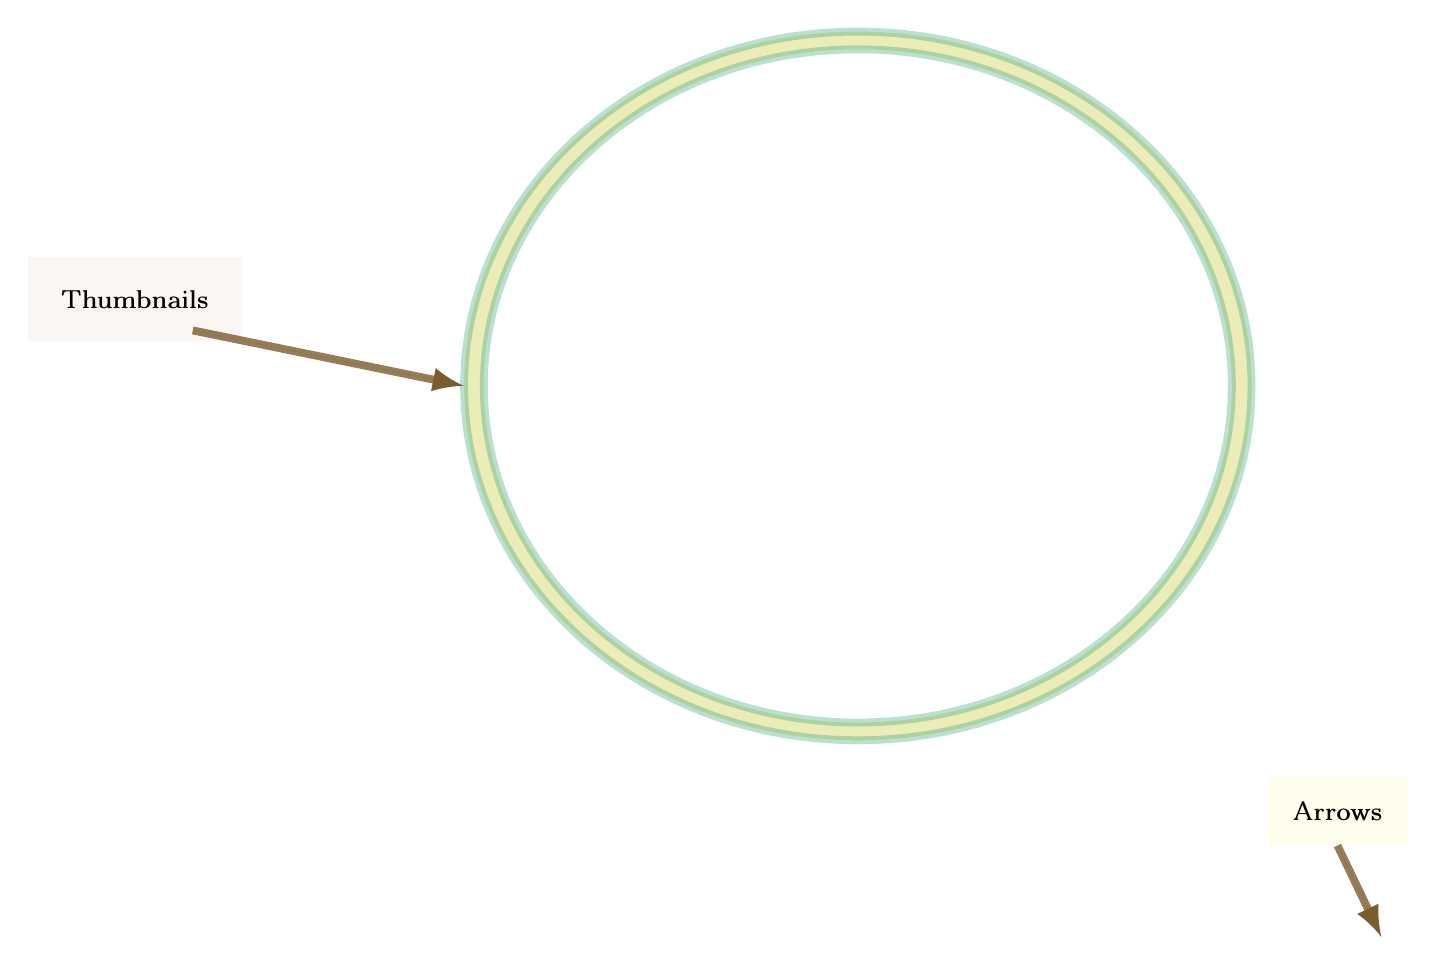
\begin{tikzpicture}
%\nodeincludegraphics[0.89\textwidth]{screenshots/ss-ph1.png}
\nodeincludegraphicsTRRS{1}{3.3cm}{3cm}{2cm}{1cm}{screenshots/ss-ph1.png}

\ann{BlueGreen}{0.3}{1mm}{grammarArrowColor}{0.5}{13.5,8}{5}{4.5}{0.95}

%\node [anchor=west] (note) at (6.25,9) {\Huge {\color{blGreen!30!black}Thumbnails}};
\node [anchor=west,fill=brown!8!white,inner sep=12, 
opacity=0.88, text opacity=1] (note) at (2.95,9.1) {\Huge {\hc{Thumbnails}}};

\colorarr{>=latex, ->}{fcBoxColor!60!black}{0.8}%
{blGreen!30!red}{1}{1mm}{[xshift=2em,yshift=.4em]note.south}{8.5, 8}

%\node [anchor=west] (noteArr) at (20.15,3) {\Huge {\color{blGreen!30!black}Arrows}};

\node [anchor=west,fill=yellow!15!white,inner sep=9, 
opacity=0.5, text opacity=1] (noteArr) at (18.7,2.6) {\hc{Arrows}};


\colorarr{>=latex, ->}{fcBoxColor!60!black}{0.8}%
{blGreen!30!red}{1}{1mm}{noteArr.south}{20.15,1}

\end{tikzpicture}


\end{frame}


%

\begin{frame}{\ft{Photo Viewer Color Coding}}

\doubleFrame{The Photo Viewer would access embedded data structures 
which specify how photos are grouped into categories, such as 
different kinds of rooms (entrance/foyer/hall, 
kitchen/dining room, bedroom, etc.).  Colors 
are assigned to each group, with 
%When rendering the thumbnail images, 
color thumbnail used as visual cues marking each
photo's classification.  Realtors can  
modify the group names and their corresponding colors,  
according to their own preferences.}

\begin{tikzpicture}
%\nodeincludegraphics[0.9\textwidth]{screenshots/ss-ph2.png}
\nodeincludegraphicsTRRS{1}{4.6cm}{2.2cm}{0.8cm}{1cm}{screenshots/ss-ph2.png}

\rectann{darkRed}{0.7}{1mm}{grammarArrowColor}{0.5}{0.05,0.5}{9.4}{5.25}{0.9}

\node [anchor=west,fill=brown!8!white,inner sep=12, 
opacity=0.88, text opacity=1] (note) at (11,2.89) {\hc{Current Photo}};

\colorarr{>=latex, ->}{fcBoxColor!60!black}
{0.8}{blGreen!30!red}{1}{1mm}{note.west}{6.58, 7.25}


\end{tikzpicture}


\end{frame}


%

\begin{frame}{\ft{Photo Viewer Interactive Cues}}

\doubleFrame{Color insertions switch from horizontal 
to vertical indicating which photos have been viewed 
(enlarged).  Separate and apart from that, the 
thumbnail of the current enlarged photo 
is marked with a thick colored border.  This border will 
surround the thumbnail and the overlay both for photos being 
viewed for the first time (with a horizontal color-band) 
and for photos being viewed a second time (with a vertical 
color-band).
}

\begin{tikzpicture}
%\nodeincludegraphics[0.9\textwidth]{screenshots/ss-ph3.png}
\nodeincludegraphicsTR{5.5cm}{3.23cm}{screenshots/ss-ph3.png}

 %%\node [anchor=west] (note) at (11,11.2) {\Huge {\color{blGreen!30!black}Already Viewed}};

\node [anchor=west,fill=brown!8!white,inner sep=12, 
opacity=0.88, text opacity=1] (note) at (7,11.8) {\hc{Already Viewed (vertical color band)}};


%\ann{BlueGreen!30!red}{1}{.8mm}{blue!50!orange}{0.5}{3.61,8.95}{.4}{.6}{0.7}

\colorarr{>=latex, ->}{fcBoxColor!20!black}
{0.8}{darkRed!70!blue}{2}{1mm}{note.west}{3.7, 9}


\node [anchor=west,fill=brown!8!white,inner sep=12, 
opacity=0.88, text opacity=1] (note) at (6.3,9.7) {\hc{Not Yet Viewed (horizontal color band)}};

%\ann{BlueGreen!30!red}{1}{.8mm}{blue!50!orange}{0.5}{7.6, 7.3}{.73}{.35}{0.7}

%
\colorarr{>=latex, ->}{fcBoxColor!20!black}
{0.8}{darkRed!70!blue}{2}{1mm}{note.south}{8.2, 7.25}

%\node [anchor=west] (note) at (11,3) {\Huge {\color{blGreen!30!black}Current Photo}};

\node [anchor=west,fill=brown!8!white,inner sep=12, 
opacity=0.88, text opacity=1] (note) at (5,1.89) {\hc{Current Photo (viewed for the second time)}};

\colorarr{>=latex, ->}{fcBoxColor!60!black}
{0.8}{blGreen!30!red}{1}{1mm}{note.north west}{4.39, 4.75}


\end{tikzpicture}


\end{frame}



%

\begin{frame}{\ft{Room Highlights Dialog Box: Room-By-Room Breakdown}}

\doubleFrame{The Re-PDF viewer provides a special 
dialog box to show the room-by-room 
breakdown of architectural/decorative features/amenities.}

\begin{tikzpicture}

%\nodeincludegraphics[0.85\textwidth]{screenshots/ss-rm1.png}
\nodeincludegraphicsTR{5.5cm}{2cm}{screenshots/ss-rm1.png}

\ann{darkRed}{0.7}{1mm}{grred!30!brown}{0.5}{13,9}{10}{3}{0.8}

\node [anchor=west,fill=white,inner sep=8]
 (note) at (13,9) {\hc{Feature Descriptions}};
 
% \node [anchor=west,fill=yellow!5!white,opacity=.95,
% text opacity=1,inner sep=9, text width=6.8]
%  (longnote) at (5,4.8) {{\color{black}{Each room features, one of which is highlighted at a %time}
%  }
%  };


 \node [anchor=west,fill=yellow!5!white,opacity=.95,
 text opacity=1,inner sep=9, text width=6.8cm]
  (longnote) at (5,4.8) {{\color{brred!30!black}{%
  {\hspace*{0.8em}\parbox{6.3cm}{
  {\LARGE {\begin{centering}\begin{spacing}{1.1}\textbf{Each room description is divided into several features, 
  one of which is highlighted at a time}\end{spacing}\end{centering}}}}}}}};
  

\end{tikzpicture}


\end{frame}


%

\begin{frame}{\ft{Room-By-Room Tab Organization}}

\doubleFrame{The Room-by-Room breakdown features a dual tabbed 
area: on the top appear the room tabs, and to the left appear 
the feature tabs.  The combination of 
currently selected room and feature tabs 
control the highlighting of details in room descriptions.  
Realtors will have the flexibility to choose which features 
to describe and which rooms to include in the breakdown.}

\begin{tikzpicture}
\nodeincludegraphicsTR{5.5cm}{3cm}{screenshots/ss-rm2.png}

\node [anchor=west,fill=white,inner sep=8]
 (note) at (10,8) {\hc{Dual Set of Tabs}};

\ann{darkRed}{0.7}{1mm}{grammarArrowColor}{0.5}{12,10.5}{6.5}{1}{0.85}

\colorarr{>=latex, ->}{fcBoxColor!20!black}
{0.8}{blGreen!30!red}{2}{1mm}{note.north}{15, 10}

\colorarr{>=latex, ->}{fcBoxColor!20!black}
{0.8}{blGreen!30!red}{1}{1mm}{note.west}{5.3, 6.2}

 \node [anchor=west,fill=brown!20!white,inner sep=21, text width=8.9cm]
  (longnote) at (8,3.5) {%  %{\color{rb!85!red}{
  {\cframedbox{\Large \textbf{The tab to the left determines which \makebox{feature} is  
highlighted, while tab on top \makebox{determines} which room is shown.}}}};

\ann{BlueGreen}{0.3}{1mm}{grammarArrowColor}{0.5}{3,6}{3}{4.5}{0.95}

\end{tikzpicture}


\end{frame}


%

\begin{frame}{\ft{Room-By-Room Navigation}}

\doubleFrame{The dual-tab functionality allows users to conveniently browse 
through different rooms in sequence, particularly 
when they are interested in honing in on 
one feature in particular.   By selecting a feature 
from the left margin, those become highlighted in 
each room description so users see it immediately.  
In this screenshot, the user selected window treatment 
as a feature to be highlighted in 
each room description.}

\begin{tikzpicture}
\nodeincludegraphicsTR{2.5cm}{2.5cm}{screenshots/ss-rm3.png}

\rectanneatdbl{darkRed}{0.7}{1mm}{grammarArrowColor}
{0.5}{3,12.5}{16}{-1.5}{2,-0.2}

\ann{red}{0.7}{1mm}{blue!50!cyan}{0.5}{12,3.65}{6.5}{1}{0.85}


\node [anchor=west,fill=white,inner sep=8]
 (note) at (10,10) {\hc{Browsing room-by-room ...}};

\colorarr{>=latex, ->}{fcBoxColor!20!black}
{0.8}{blGreen!30!red}{2}{1mm}{note.north west}{7.6, 11.4}

\node [anchor=west,fill=white,inner sep=8]
 (note) at (10,5.5) {\hc{and feature-by-feature ...}};

\colorarr{>=latex, ->}{fcBoxColor!60!black}
{0.8}{darkRed!70!blue}{1}{1mm}{note.west}{5.3, 4.1}


\end{tikzpicture}


\end{frame}





\begin{frame}{\ft{Using Virtual Tours}}

\doubleFrame{Another kind of dialog box is an 
embedded WebGL viewer showing  
a property\curlyapos{}s Materport tour in a detached window}

\begin{tikzpicture}
\nodeincludegraphicsTR{2.1cm}{2cm}{screenshots/ss-vt1.png}

\node [anchor=west,fill=brown!8!white,inner sep=4, 
opacity=0.88, text opacity=1]
 (note) at (10,8) {\hc{Matterport \curlyquote{Line of Sight}}};

\colorarr{>=latex, ->}{fcBoxColor!20!black}
{0.8}{blGreen!30!red}{2}{1mm}{note.south}{14.5, 5.9}


\end{tikzpicture}


\end{frame}


%

\begin{frame}{\ft{Virtual Tour Windows}}

\doubleFrame{Compared to browser-based Virtual Tours,
the embedded WebGL viewers in Re-PDF are more convenient, because 
they allow the tour window to be visually juxtaposed with 
other windows, such as the room-by-room breakdown of 
descriptions and features.}

\begin{tikzpicture}
\nodeincludegraphicsTR{2.1cm}{2cm}{screenshots/ss-vt2.png}

 \node [anchor=west,fill=yellow!10!red!2!white,opacity=0.98,
 text opacity=1,inner sep=16, text width=6cm]
  (longnote) at (14,11.15) {{\color{brred!50!black}{%
  {\hspace*{0.8em}\parbox{5.7cm}{
  {\LARGE {\begin{centering}\begin{spacing}{1.1}\textbf{Room description features
  can be linked to Matterport views of each room}\end{spacing}\end{centering}}}}}}}};

\colorarr{>=latex, ->}{fcBoxColor!20!black}
{0.8}{darkRed!70!blue}{2}{1mm}{longnote.west}{12.5, 10.5}

\colorarr{>=latex, ->}{fcBoxColor!60!black}
{0.8}{blGreen!30!red}{1}{1mm}{longnote.south}{18.5, 7.5}

\end{tikzpicture}


\end{frame}


%

\begin{frame}{\ft{Virtual Tour Tag Posts}}

\doubleFrame{With Materport tours that employ tag-posts, 
the Virtual Tour can also be synchronized 
with other parts of the application --- for 
example, showing information about a particular room when 
users click on a tag-post hyperlink positioned 
at the center of the room as depicted in a virtual tour.
Matterport spaces often use tag-posts to 
describe property features/amenities found at 
specific points in the virtual tour. 
}

\begin{tikzpicture}

\nodeincludegraphicsTRRS{1}{0cm}{1cm}{2.8cm}{3cm}{screenshots/ss-vt3.png}

%\ann{BlueGreen!30!red}{0.8}{0.7mm}{red!30!blue}{0.5}{11,4.5}{2}{2.5}{0.95}

%\polyann{BlueGreen!30!red}{0.8}{0.7mm}{red!30!blue}{0.5}{11,4.5}{6}{3cm}{3.5cm}

%\polyann{black}{1}{2mm}{red!30!blue}{0.5}{11,4.5}{6}{3cm}{3.5cm}

%\path [draw=#1,draw opacity=#2,line width=#3, fill=#4, fill opacity = #5, even odd rule] %
%	node [minimum size=#8,regular polygon,regular polygon sides=#7] at (#6) {}
%	node [minimum size=#9,regular polygon,regular polygon sides=#7] at (#6) {};}
%\path [draw=black,line width=3mm,fill=red,even odd rule] %
%	

\node [minimum size=4.2cm,regular polygon,regular polygon sides=6,
rotate=30,draw=BlueGreen!30!red,line width=1mm] (innr) at (8.3,5.58) {};

\node [minimum size=4.8cm,regular polygon,regular polygon sides=6,
rotate=30,draw=BlueGreen!30!red,line width=1mm] (outr) at (8.3,5.58) {};

\path [fill=red!30!blue,fill opacity=0.5,even odd rule]
(outr.corner 1) -- (outr.corner 2) -- (outr.corner 3) -- 
(outr.corner 4) -- (outr.corner 5) -- (outr.corner 6)
(innr.corner 1) -- (innr.corner 2) -- (innr.corner 3) -- 
(innr.corner 4) -- (innr.corner 5) -- (innr.corner 6)
;

\node [anchor=west,fill=white,inner sep=8]
 (note) at (-0.1,6) {\hc{Tag Posts}};

\node [anchor=west,fill=white,inner sep=4, text width=5.2cm]
 (longnote) at (-0.1,2.4) {{\color{rb!80!red}{%
 {\LARGE {\begin{spacing}{0.9}\textit{Matterport Tag Posts add details to fixed 
 locations in a virtual tour.  Tag Posts can include 
 text, audio, video, or hyperlinks}\end{spacing}}}}}};


\colorarr{>=latex, ->}{fcBoxColor!70!blue}{1}
{fcBoxColor!30!red}{1}{2mm}{note.east}{7.4,4.75}



%\filldraw[fill=red]
%node [minimum size=2cm,regular polygon,regular polygon sides=6,draw=black,thick]
% (innr) at (10,4.5) {}
%node [minimum size=3cm,regular polygon,regular polygon sides=6,draw=black,thick] at (10,4.5)  %(outr) {};


%\fill[even odd rule] innr outr {};
%
%\path [draw=black,line width=3mm,fill=red,even odd rule]

%
%\path[fill=red,even odd rule]
%\draw[fill, fill=red,even odd rule]

%\node [minimum size=3cm,regular polygon,
%regular polygon sides=6,draw=black,thick] (outr) at (15,4.5) {};
%\node [minimum size=2cm,regular polygon,
%regular polygon sides=6,draw=black,thick] (innr) at (15,4.5) {};

%%,save path=innr

%\path[fill=red,even odd rule]
%restore spath=innr;



%\path[fill=red,even odd rule]
%regular polygon [minimum size=3cm,regular polygon sides=6] at (15,4.5) {} 
%regular polygon [minimum size=2cm,regular polygon sides=6] at (15,4.5) {};


%\ann{BlueGreen!30!red}{0.8}{0.7mm}{red!30!blue}{0.5}{11,4.5}{2}{2.5}{0.95}

\end{tikzpicture}


\end{frame}



%

\begin{frame}{\ft{Using MeshLab and Panini with the Re-PDF Viewer}}

\doubleFrame{Realtors can also opt to export their 
Matterport \curlyquote{dollhouse} to MeshLab (a 3D graphics engine) 
and their panorama-photos to Panini (a viewer for many 
panorama geometries).  Both of these applications can 
be customized and bundled 
with Re-PDF software.}

\begin{tikzpicture}
\nodeincludegraphicsTRRS{1.2}{13.16cm}{1cm}{4cm}{4cm}{screenshots/snapshot07.png}
\end{tikzpicture}

\end{frame}


%

\begin{frame}{\ft{Deleting Saved Files}}

\doubleFrame{After users study a property, they have the option of 
removing the local files that were extracted from the PDF 
document when it was first opened in the Re-PDF application.}

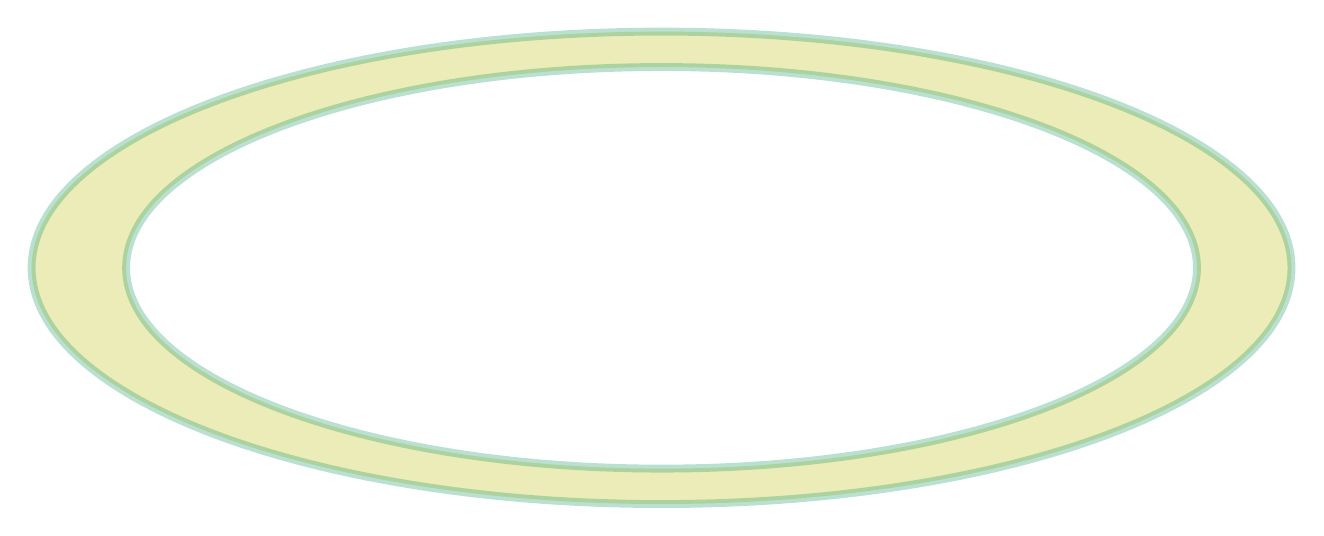
\begin{tikzpicture}
\nodeincludegraphicsTRRS{1}{3.83cm}{0cm}{3.7cm}{0cm}{screenshots/ss-cl2.png}

\ann{BlueGreen}{0.3}{1mm}{grammarArrowColor}{0.5}{12,8}{8}{3}{0.85}

\end{tikzpicture}

\end{frame}



\end{document}
